\documentclass[12pt]{article}

\usepackage[left=1.9cm, right=1.27cm, top=1.52cm, bottom=2.5cm]{geometry} 
\usepackage[utf8]{inputenc}
\usepackage[titletoc,title]{appendix} % Adding appendices 
\usepackage{sectsty} %For changing section/header styles 
\usepackage[english]{babel}
\usepackage{helvet} 
\usepackage{ulem} 
\usepackage{listings}
\usepackage{fancyhdr}
\usepackage{graphicx}

\graphicspath{ {images/} }

% Header styling
\fancypagestyle{titlePage}{ 
    \fancyhf{}
    \fancyfoot[L]{Capstone\_7790\_01\_ANR\_template\_201630.docx} 
    \fancyfoot[R]{\today}
    \renewcommand{\headrulewidth}{0pt} 
}

\fancypagestyle{neilReport}{ 
    \fancyhf{} 
    \fancyhead[L]{\footnotesize BCIT ELEX 7790: Capstone Project Initiation} 
    \fancyhead[R]{ANR: Short title and version \# goes here}
    \fancyfoot[L]{filename} 
    \fancyfoot[C]{\thispage of }
    \fancyfoot[R]{\today} 
}

\renewcommand{\footrulewidth}{1pt}

% change style of abstract environment
\renewenvironment{abstract} {
\centering
    
    {\fontsize{16pt}{12pt}\fontfamily{qpl}\selectfont\itshape \abstractname}

\flushleft
}
{}


% Section styling
\sectionfont{\sffamily\bfseries\fontsize{16pt}{0pt}}
\subsectionfont{\sffamily\bfseries\itshape\fontsize{14pt}{0pt}}
\subsubsectionfont{\sffamily\bfseries\fontsize{13pt}{0pt}}

% Paragraph spaceing
\setlength{\parindent}{0em}
\setlength{\parskip}{0.5em}

% header and footer spacing
\setlength{\headheight}{36pt}
\setlength{\headsep}{12pt}
\setlength{\footskip}{32pt}

\begin{document} 

\thispagestyle{titlePage}


\includegraphics[scale=0.12]{BCIT}
\bigskip

\begin{center}
    
    {\fontsize{24pt}{6pt}\fontfamily{qpl}\selectfont ELEX 7815: Digital Image \& Video Processing}
    
    \vspace{12pt}
    
    {\fontsize{28pt}{12pt}\fontfamily{qpl}\selectfont\bfseries Lab 1}
    
    \vspace{12pt}
    
    {\fontsize{26pt}{12pt}\fontfamily{qpl}\selectfont\bfseries\itshape Image Manipulation}
    
    \vspace{12pt}
    
    {\fontsize{16pt}{12pt}\fontfamily{qpl}\selectfont\underline{\date}}}
    
    \vspace{24pt}

\end{center}

\begin{abstract}

This lab focuses on the mechanisms in which Matlab loads, saves, and manipulates
images. First simple loading and saving was experimented with, and an image was
compared at varying degrees of quality. Next was an exploration of RGB color
representation where an image was broken down into its three color channels as
well as translated into an indexed image. Autocorrelation of a single row was
done at the end of the lab, it was concluded that compression algorithms likely
use correlation in order to detect repeating patterns within images.

\end{abstract}


\pagebreak

\pagestyle{neilReport}

\tableofcontents

\pagebreak

\section{Task 1: Reading and Writing Grayscale Images}

The first step in this lab is to load an image using imread. When Matlab loads
an image , it takes th image file, whatever format it is saved in, and stores
the raw image data in a two-dimension array. We want to end the line containing
the call to imread with a semicolon so that it does not print the value of every
pixel to the console. We also can extract additional information on our first
image, barbara.jpg, using functions iminfo, whos, and size. The
console output is shown below:

\begin{itemize}

    \item \textbf{iminfo:}
    
    \lstinputlisting{../iminfoDump.txt}

    \item \textbf{whos:}

    \lstinputlisting{../whosDump.txt}

    \item \textbf{size:}

    \lstinputlisting{../sizeDump.txt}

\end{itemize}

So here we can see that barbara is a 256x256 image made up of uint8 (unsigned
8-bit integers).

In order to view barbara we use imshow. Providing only the image object as an
argument simply displays the image, but if we also provide a 1x2 matrix [a, b]
the function will make all pixels with an intensity less than a black and all
pixels above b to be white. Providing an empty matrix performs auto contrast
adjustment, transforming intensity values to maximize contrast without losing
information.

\begin{figure}[H]
    \centering
    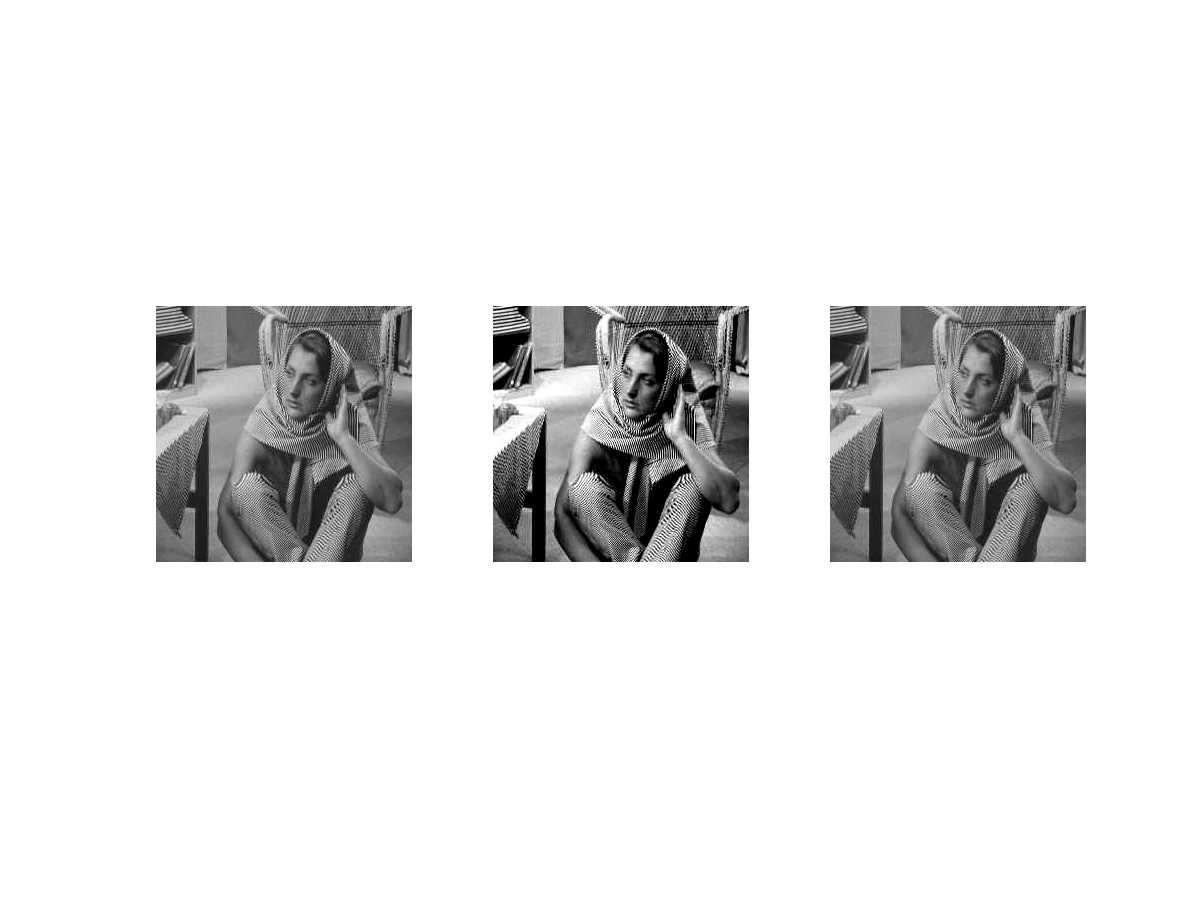
\includegraphics[scale=0.5]{imshow}
    \caption{Output of imshow providing nothing, [a, b], and [] for the second
    argmument}
\end{figure}

The imtool function can be used to zoom into the chosen image, view pixel
intensity values, and alter them. I used this function to explore some of the
values in barbara, alter them, and see the affect of those changes zoomed out.

In Matlab we can save image objects to a file using imwrite and we can save them
under different quality levels. In this example we save lena.tiff and see the
effects of saving it at different quality levels:

\begin{figure}[H]
    \centering
    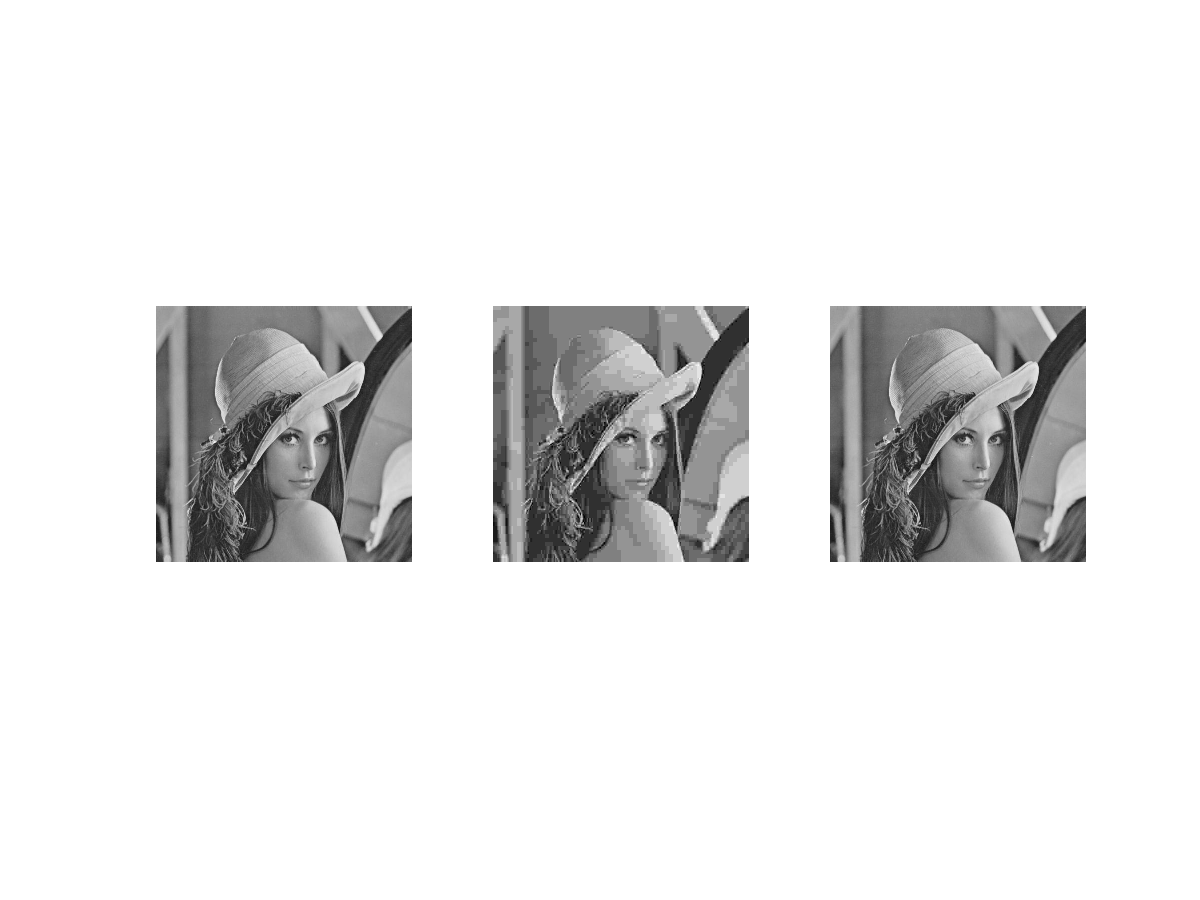
\includegraphics[scale=0.5]{lenaCompare}
    \caption{Comparison of lena saved at different qualities}
\end{figure}

The images are saved at smaller sizes when quality is decreased. For example,
lena3 is 32x32. Matlab seems to view lena3 at the same size as the other two
images, and hence applied a scaling transformation to do so (probably using
linear interpolation). This is why we are not viewing it as large pixels, but a
very blurry image.


\section{Task 2: Reading Color Images}

Now it's time to look at some color images. First we have fruits.png:

\begin{figure}[H]
    \centering
    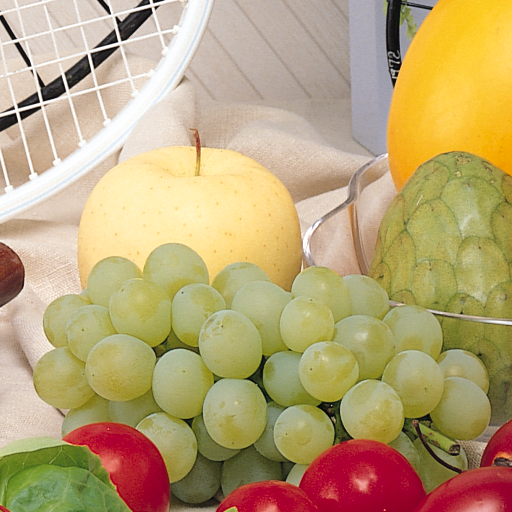
\includegraphics[scale=0.5]{fruits}
    \caption{Original fruits.png image}
\end{figure}

This image is a (mxnx3) image because it has three channels: Red, Green, and
Blue. For example, if we look at pixel (93,180) we get a value of (r,g,b),
again, each value represents Red, Green, and Blue intensities. If we separate
the image into its induvidual channels we get the following:

\begin{figure}[H]
    \centering
    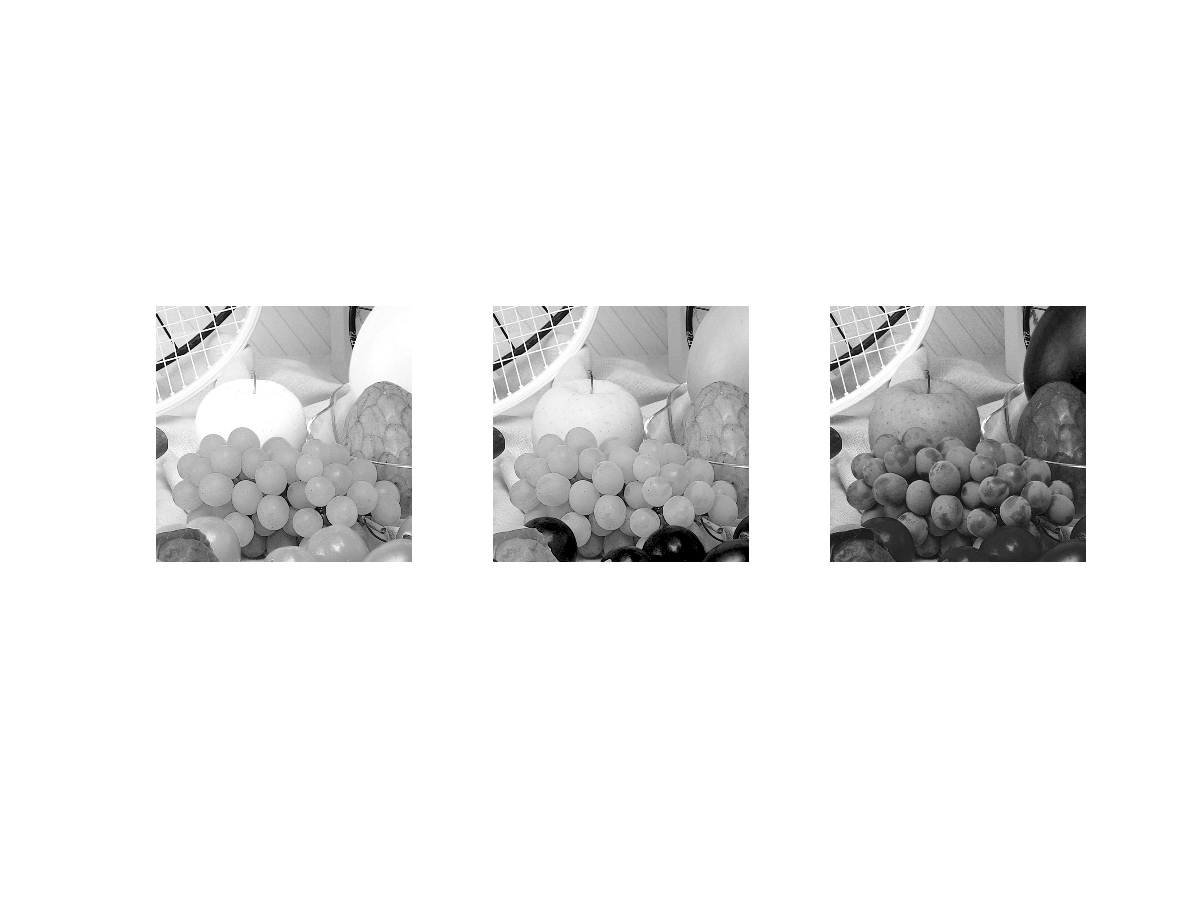
\includegraphics[scale=0.5]{threeChannels}
    \caption{Red, Green, and Blue channels of fruits.png}
\end{figure}

While the above images are in black and white, they represent the intensities of
their respective colors, so white in the "red" channel represents the red maximm
intensity of red. A white pixel in the original fruits image will be seen as
white in all three channels, as it is the max value for red, green, and blue.

Now I will convert fruits into an indexed image, I will index it with 16 and 256
colors. Indexed images can significantly reduce the memory taken up by an image
when there are few colors in said image. It does this by making an indexed table
of colors, the raw image data then becomes a single index value (instead of RGB)
which points to an RGB value in the table.

\begin{figure}[H]
    \centering
    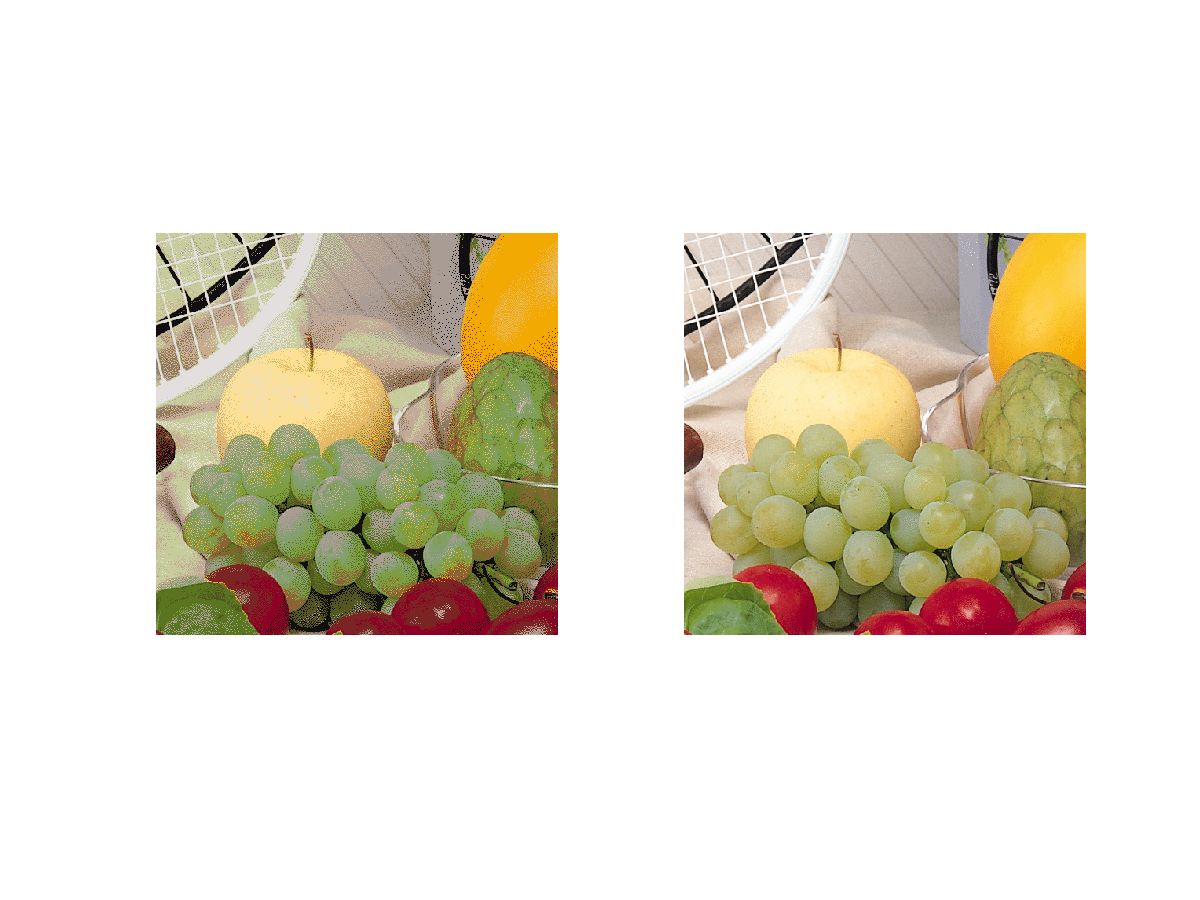
\includegraphics[scale=0.5]{indexed}
    \caption{256 and 16 indexed color image of fruits}
\end{figure}

If an image has many colors, the table can be made to be large to accomodate all
the colors, but then the indexed image does not save nearly as much memory,
which is the whole point of indexing! Alternatively the color table is kept
small, and much of the imformation in the image is lost. That is exactly what we
see in the above figure with 256 and 16 color indexing.
 

\input{task3} 

\section{Task 4: Pixel Intensity Along One Row and its Correlation}

Now let's plot the intensities of row 164 of cameraman.tif. The full image is
also provided for reference.

\begin{figure}[H]
    \centering
    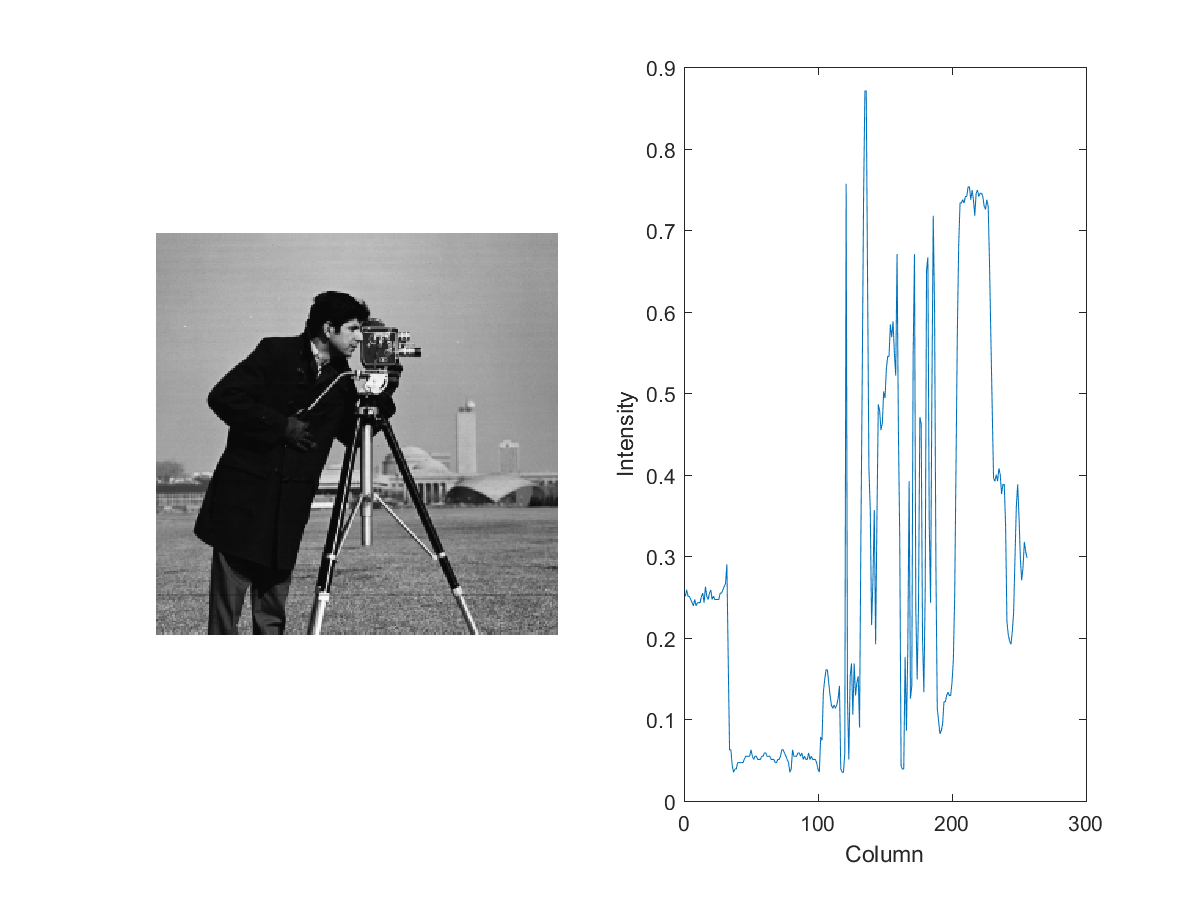
\includegraphics{rowIntensity}
    \caption{cameraman.tif and Row Intensity}
\end{figure}

There looks like there might be some correlation as we seem to be transitioning
between two intensity ranges of the foreground and background. Let's perform
autocorrelation.

\begin{figure}[H]
    \centering
    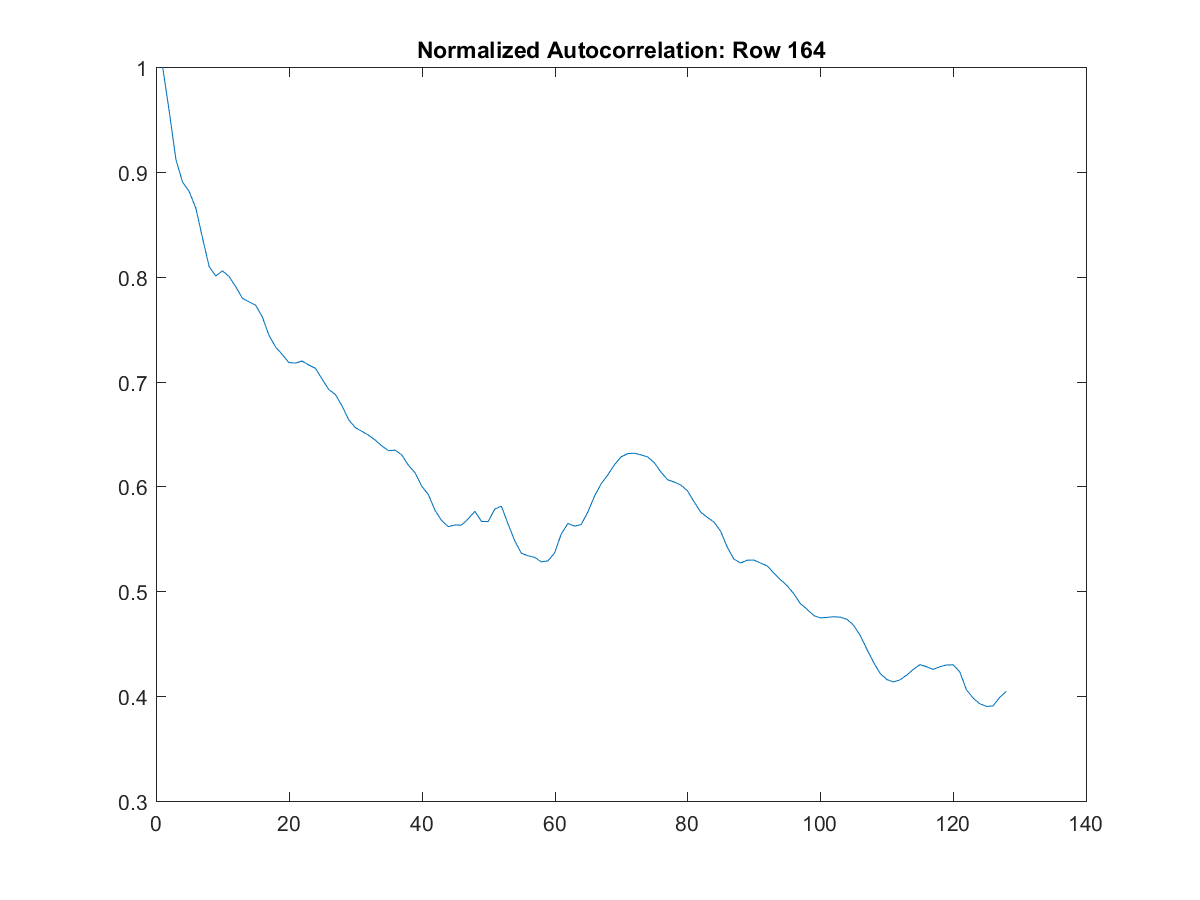
\includegraphics{autocorrelation}
    \caption{Autocorrelation of Row 164}
\end{figure}

In this case, autocorrelation starts with the signal fully overlapping itself
(and therefore correlation coefficient starts at 1). The signals are then only shifted
over half the range of the image. This is because the correlation signal would
mirror itself otherwise, and we only need to see the important information.

Continuing from earlier, we can see that there is a local peak of correlation
around column X. given the shape of this image we would likely find more
correlation in the colimns as many of the shapes are skinny and tall, and
therefore constant in value.

It is likely that many compression algorithms use correlation. If an image has a
repeating pattern, then we really only need to record that pattern once. I also
image that basic image data compression algorithms check for greater correlation
in the horizontal and vertical directions. This would account for cases where an
image is highly correlated in one direction but not the other.


\section{Conclusion}

In ths lab we thoroughly examined the mechanisms in which Matlab loads, saves,
and manipulates image data. Matlab does provide a convenient platform in which
to experiment with and implement image processing. 

The functions and methods used in this lab will clearly be used throughout the
course. It was extremely important for us to manually go through some of the
images and inspected their values. Separating an image into its RGB channels was
very illustrative, as well as playing around with the indexing functionality.

Task 4 provided some challenge for writing Matlab scripting which was a good way
to end things off since now we will be doing more advanced operations on images.
 

\end{document}
